% Created 2021-02-12 vie 18:36
% Intended LaTeX compiler: pdflatex
\documentclass[presentation,aspectratio=169]{beamer}
\usepackage[utf8]{inputenc}
\usepackage[T1]{fontenc}
\usepackage{graphicx}
\usepackage{grffile}
\usepackage{longtable}
\usepackage{wrapfig}
\usepackage{rotating}
\usepackage[normalem]{ulem}
\usepackage{amsmath}
\usepackage{textcomp}
\usepackage{amssymb}
\usepackage{capt-of}
\usepackage{hyperref}
\usepackage{khpreamble}
\usepackage{amssymb}
\usepgfplotslibrary{groupplots}
\usepackage{gensymb}
\newcommand*{\shift}{\operatorname{q}}
\usetheme{default}
\author{Kjartan Halvorsen}
\date{2021-02-15}
\title{Encoder incremental}
\hypersetup{
 pdfauthor={Kjartan Halvorsen},
 pdftitle={Encoder incremental},
 pdfkeywords={},
 pdfsubject={},
 pdfcreator={Emacs 26.3 (Org mode 9.4.4)}, 
 pdflang={English}}
\begin{document}

\maketitle

\section{Encoder}
\label{sec:org432b10b}

\begin{frame}[label={sec:org044eded}]{Encoder incremental}
\begin{center}
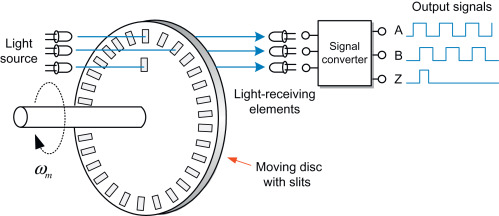
\includegraphics[width=0.7\textwidth]{../../figures/encoder-im.jpg}
{\footnotesize Fuente: \url{https://www.sciencedirect.com/topics/engineering/incremental-encoder}}
\end{center}
\end{frame}

\begin{frame}[label={sec:org6b2e07b}]{Encoder incremental}
\begin{center}
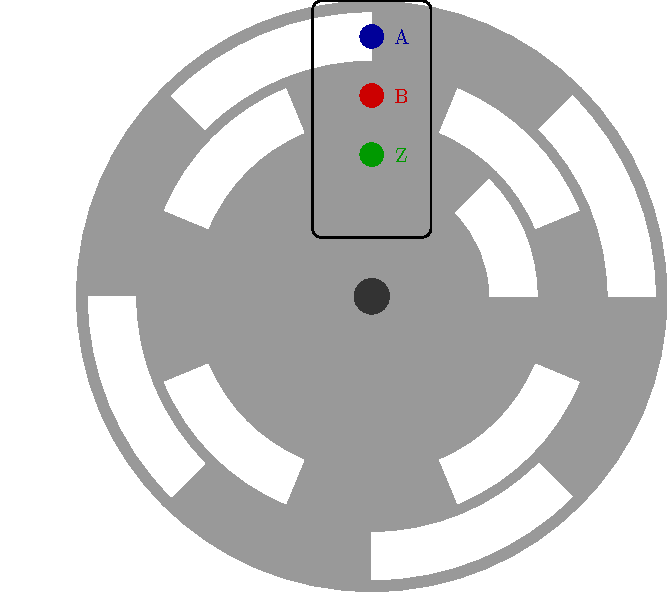
\includegraphics[width=0.4\textwidth]{../../figures/encoder-disc}
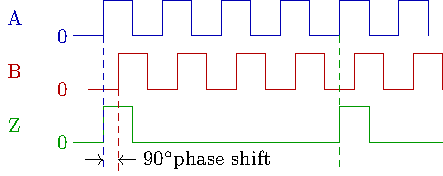
\includegraphics[width=0.5\textwidth]{../../figures/encoder-signals}
\end{center}

\emph{Pulses Per Revolution (PPR)} es igual a 4 en el ejemplo. Cada apertura tiene un sector de \(\frac{360\degrees}{2 \times PPR} = 45\degree\).
\end{frame}

\begin{frame}[label={sec:org7cca9f2}]{Encoder incremental}
\begin{center}
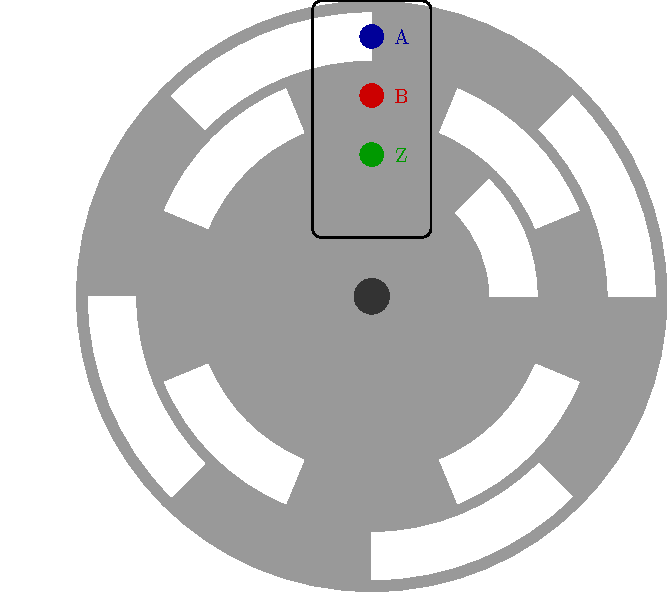
\includegraphics[width=0.4\textwidth]{../../figures/encoder-disc}
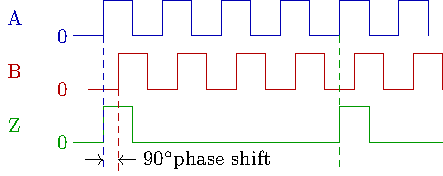
\includegraphics[width=0.5\textwidth]{../../figures/encoder-signals}
\end{center}

\alert{Actividad individual} Si detectamos los flancos positivos \alert{y} los flancos negativos de las dos señales \textcolor{blue!80!black}{A} y \textcolor{red!80!black}{B}. Cual sería el giro minimo que podemos detectar (la sensitivad del sensor)?
\end{frame}


\begin{frame}[label={sec:org127e9ad}]{Encoder incremental}
\begin{center}
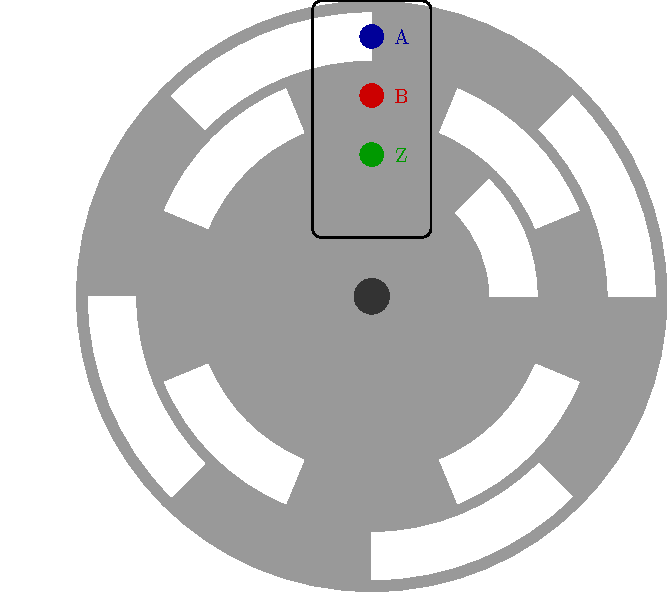
\includegraphics[width=0.4\textwidth]{../../figures/encoder-disc}
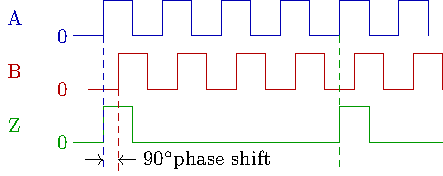
\includegraphics[width=0.5\textwidth]{../../figures/encoder-signals}
\end{center}

\alert{Actividad individual} En el ejemplo arriba, el sensor gira en sentido del reloj (CW) o en sentido contrario al reloj (CCW)?
\end{frame}


\begin{frame}[label={sec:org454d780}]{Encoder incremental}
\begin{center}
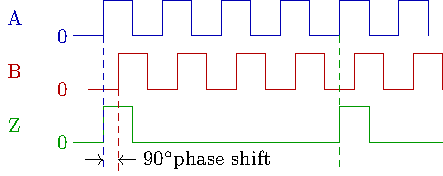
\includegraphics[width=0.5\textwidth]{../../figures/encoder-signals}

\begin{tikzpicture}
  \begin{axis}[
    width=8cm,
    height=4cm,
    ]
    \addplot[const plot, no markers, 0:5, samples=20] { 1.0/(1 + exp(-x))};
    };
  \end{axis}
\end{tikzpicture}
\end{center}
\end{frame}
\end{document}